\documentclass[10pt,twocolumn,letterpaper]{article}

% Buildable two-column development layout. Replace only the class and venue
% boilerplate when the official ICRA 2027 author kit becomes available.
\usepackage[T1]{fontenc}
\usepackage[utf8]{inputenc}
\usepackage{lmodern}
\usepackage{microtype}
\usepackage[margin=0.68in,top=0.72in,bottom=0.82in]{geometry}
\usepackage{graphicx}
\usepackage{booktabs}
\usepackage{tabularx}
\usepackage{array}
\usepackage{multirow}
\usepackage{placeins}
\usepackage{flushend}
\usepackage{amsmath,amssymb}
\usepackage{xcolor}
\usepackage{enumitem}
\usepackage{tikz}
\usetikzlibrary{arrows.meta,backgrounds,calc,fit,positioning,shapes.geometric}
\usepackage[hidelinks]{hyperref}
\usepackage[numbers,sort&compress]{natbib}
\usepackage{mciteplus}
\mciteErrorOnUnknownfalse

\definecolor{AuditBlue}{HTML}{356A8A}
\definecolor{ActionTeal}{HTML}{21867A}
\definecolor{GainOrange}{HTML}{D97732}
\definecolor{SafetyRed}{HTML}{B7473A}
\definecolor{SoftGray}{HTML}{EEF1F3}
\definecolor{DarkGray}{HTML}{3D454D}

\newcommand{\method}{VCA-Filter}
\newcommand{\Aaction}{\mathcal{A}_{\mathrm{action}}}
\newcommand{\Aaudit}{\mathcal{A}_{\mathrm{audit}}}
\newcommand{\etal}{\textit{et al.}}
\newcolumntype{Y}{>{\raggedright\arraybackslash}X}
\makeatletter
\def\bstctlcite{\@ifnextchar[{\@bstctlcite}{\@bstctlcite[@auxout]}}
\def\@bstctlcite[#1]#2{\@bsphack
  \@for\@citeb:=#2\do{%
    \edef\@citeb{\expandafter\@firstofone\@citeb}%
    \if@filesw\immediate\write\csname #1\endcsname
      {\string\citation{\@citeb}}\fi}%
  \@esphack}
\makeatother
\setlength{\columnsep}{0.24in}
\setlength{\textfloatsep}{7pt plus 2pt minus 2pt}
\setlength{\floatsep}{6pt plus 2pt minus 2pt}
\setlist{nosep,leftmargin=*}

\title{Visual-Conditioned Continuous Action Filtering for\\
Auditable Robot Teleoperation Data Collection}
\author{Anonymous Authors}
\date{}

\begin{document}
\raggedbottom
\bstctlcite{paper:BSTcontrol}
\maketitle

\begin{abstract}
The bottleneck in collecting real-robot data is not only volume, but whether
demonstrations are valid, auditable, and useful for downstream policy learning.
In visually observable tasks that require local alignment or short-horizon
refinement, useful data include both smooth nominal executions and sparse,
timely corrections in difficult states. Novice operators, however, may spend
substantial time obtaining only a few valid demonstrations. We present a
visual-conditioned continuous action filter for teleoperation and organize it
within an iterative data-collection loop. The system synchronously records raw
operator commands, robot state, and multi-view images. Successful nominal
segments and human-confirmed correction intervals form complementary
supervision, while a frozen visual encoder and an offline vision-language model
support phase and progress auditing. A causal temporal model uses separate
heads for a conditional expert-action distribution and a bounded,
rate-constrained assistance gain. Their outputs form a bounded residual that
continuously modulates the operator command. Our real-robot evaluation measures
audit quality, assistance behavior and generalization, valid demonstrations per
operator minute, and downstream imitation-learning utility. A frozen reference
audit set and independent per-round review are used to distinguish genuine
collection gains from audit drift across iterations.

\end{abstract}

\section{Introduction}
\label{sec:introduction}

Embodied policy learning increasingly depends on the quality and downstream
utility of demonstrations, rather than on record count alone
\citep{yeDataPyramidEmbodied2026,hejnaRobotDataCuration2025,hoqueEGODEXLEARNINGDEXTEROUSMANIPULATION2026,collaborationOpenXEmbodimentRobotic2025}.
Simulation, portable teleoperation, egocentric recording, and large-scale
real-robot datasets have broadened the sources of manipulation data
\citep{collaborationOpenXEmbodimentRobotic2025,chiUniversalManipulationInterface2024,khazatskyDROIDLargeScaleInTheWild2024,hoqueEGODEXLEARNINGDEXTEROUSMANIPULATION2026,mandlekarMimicGenDataGeneration2023}.
Yet these collection paradigms do not share a common record of temporal
synchronization, task phase, operator correction, and failure cause. Recent
visual auditing and reward-modeling methods begin to represent failures,
progress, near misses, and partial completion explicitly
\citep{duanAHAVisionLanguageModelDetecting2024,leeRoboRewardGeneralPurposeVisionLanguage2026,sermanetRoboVQAMultimodalLongHorizon2024,wuLargeRewardModels2026}.
For visually observable manipulation with tight action tolerances,
misalignment, stagnation, and repeated attempts reduce the reuse value of a
demonstration. Data curation and visuomotor policy studies likewise show that
trajectory properties and data selection affect downstream learning
\citep{hejnaRobotDataCuration2025,chiDiffusionPolicyVisuomotor2024,zhaoLearningFineGrainedBimanual2023}.

High-quality demonstrations do not require assistance at every step. Smooth,
single-pass executions preserve the operator's nominal behavior, while local
corrections reveal how an expert recovers from difficult states
\citep{rossReductionImitationLearning2011,liuRobotLearningJob2023,luoPreciseDexterousRobotic}.
Current work covers the required components separately: teleoperation systems
address how demonstrations are collected
\citep{wuGELLOGeneralLowCost2024,chengOpenTeleVisionTeleoperationImmersive2024,wangDexCapScalablePortable2024,qinAnyTeleopGeneralVisionBased2024,xuDexUMIUsingHuman2025};
data-quality and visual models score trajectories after collection
\citep{hejnaRobotDataCuration2025,duanAHAVisionLanguageModelDetecting2024,leeRoboRewardGeneralPurposeVisionLanguage2026};
and shared control, residual learning, and interactive imitation learning
primarily optimize deployment success or expert-intervention cost
\citep{johanninkResidualReinforcementLearning2019,javdaniSharedAutonomyHindsight2015,hoqueThriftyDAggerBudgetAwareNovelty2021,welteFlowCorrectEfficientInteractive2026a}.
What remains unclear is whether audited historical demonstrations can improve
the yield of the \emph{next} teleoperation round under fixed operator-time and
safety budgets, while preserving operator commands in nominal states.

We study this question through a causal, visual-conditioned continuous action
filter. Correction intervals provide weak supervision for difficult portions
of a trajectory; successful nominal segments constrain unnecessary action
offsets. A frozen visual encoder supplies continuous observations, and an
offline vision-language auditor proposes phase, progress, stagnation, and
recovery events for human review. The online model predicts a candidate expert
action and a time-varying assistance gain. Their difference from the raw human
command produces a bounded residual whose strength changes gradually with task
context. Executing the filtered command produces the next visual observation,
and newly audited episodes supply the next training round. Fig.~\ref{fig:overview}
summarizes this loop.

\begin{figure*}[t]
  \centering
  \resizebox{0.99\textwidth}{!}{%
  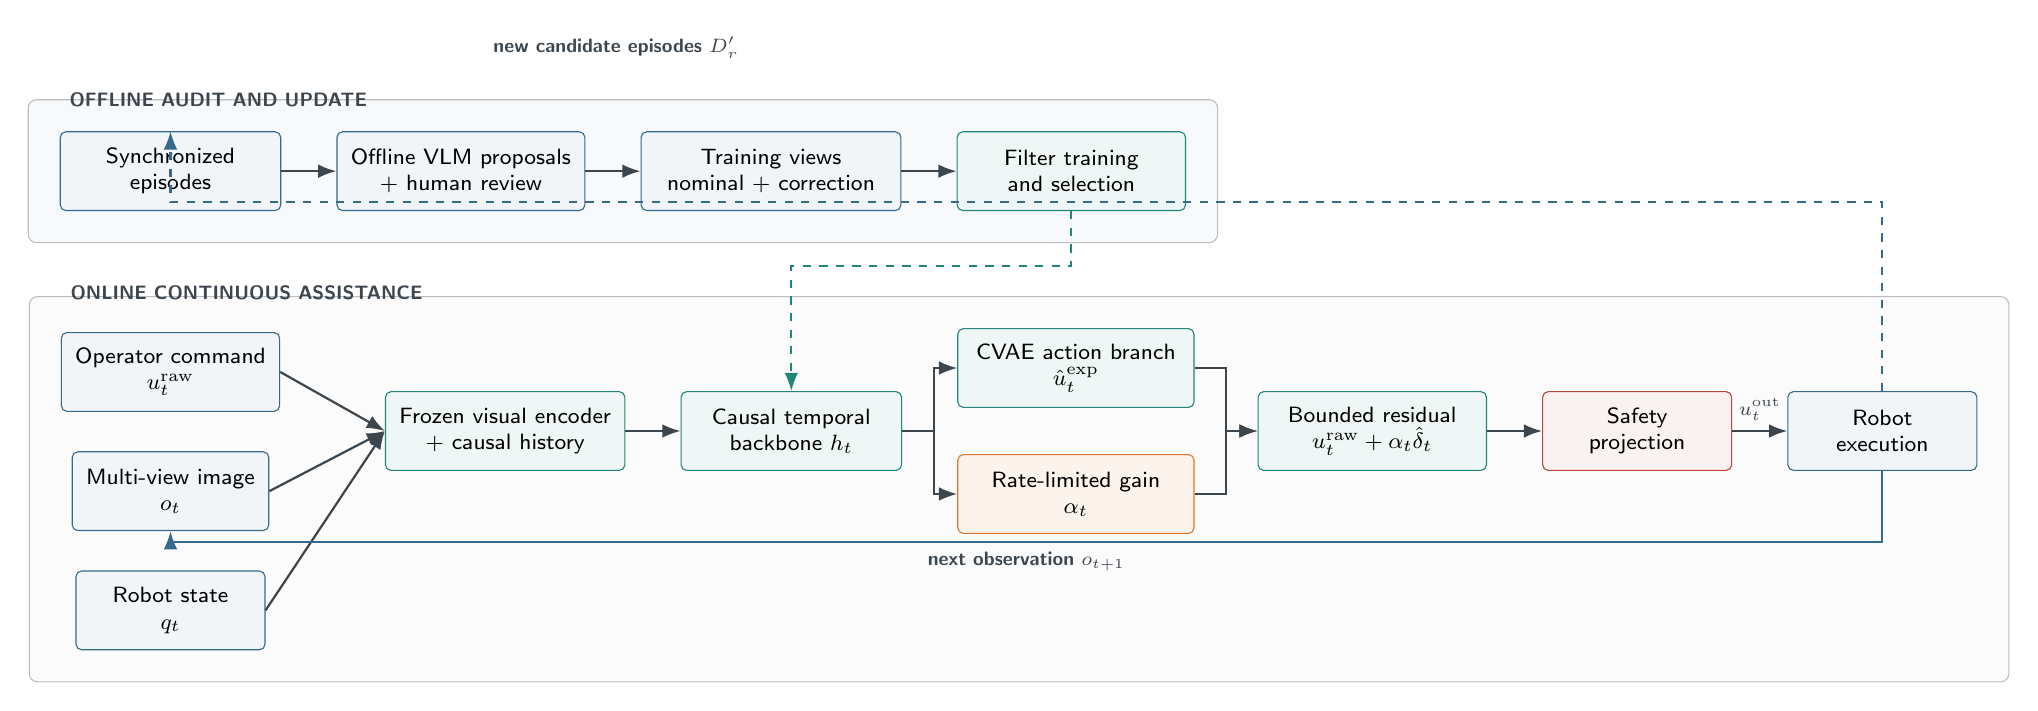
\begin{tikzpicture}[
    font=\sffamily\footnotesize,
    >=Latex,
    flow/.style={->,line width=0.8pt,draw=DarkGray},
    data/.style={draw=AuditBlue,fill=AuditBlue!7,rounded corners=2pt,
      minimum height=10mm,align=center,inner xsep=5pt},
    model/.style={draw=ActionTeal,fill=ActionTeal!7,rounded corners=2pt,
      minimum height=10mm,align=center,inner xsep=5pt},
    gain/.style={draw=GainOrange,fill=GainOrange!9,rounded corners=2pt,
      minimum height=10mm,align=center,inner xsep=5pt},
    safety/.style={draw=SafetyRed,fill=SafetyRed!7,rounded corners=2pt,
      minimum height=10mm,align=center,inner xsep=5pt},
    tag/.style={font=\sffamily\scriptsize\bfseries,text=DarkGray}
  ]
    % Offline audit and update path.
    \node[data,minimum width=28mm] (episodes) at (0,2.55)
      {Synchronized\\episodes};
    \node[data,minimum width=31mm,right=7mm of episodes] (audit)
      {Offline VLM proposals\\+ human review};
    \node[data,minimum width=33mm,right=7mm of audit] (views)
      {Training views\\nominal + correction};
    \node[model,minimum width=29mm,right=7mm of views] (train)
      {Filter training\\and selection};
    \draw[flow] (episodes) -- (audit);
    \draw[flow] (audit) -- (views);
    \draw[flow] (views) -- (train);
    \node[tag,anchor=west] at ($(episodes.north west)+(0,4mm)$)
      {OFFLINE AUDIT AND UPDATE};

    % Online input path.
    \node[data,minimum width=24mm] (human) at (0,0)
      {Operator command\\$u_t^{\mathrm{raw}}$};
    \node[data,minimum width=24mm,below=5mm of human] (vision)
      {Multi-view image\\$o_t$};
    \node[data,minimum width=24mm,below=5mm of vision] (state)
      {Robot state\\$q_t$};

    \node[model,minimum width=28mm] (context) at (4.25,-0.75)
      {Frozen visual encoder\\+ causal history};
    \node[model,minimum width=28mm,right=7mm of context] (backbone)
      {Causal temporal\\backbone $h_t$};
    \node[model,minimum width=30mm,right=7mm of backbone,yshift=8mm] (action)
      {CVAE action branch\\$\hat u_t^{\mathrm{exp}}$};
    \node[gain,minimum width=30mm,right=7mm of backbone,yshift=-8mm] (gain)
      {Rate-limited gain\\$\alpha_t$};
    \node[model,minimum width=29mm,right=8mm of action,yshift=-8mm] (compose)
      {Bounded residual\\$u_t^{\mathrm{raw}}+\alpha_t\hat\delta_t$};
    \node[safety,minimum width=24mm,right=7mm of compose] (safe)
      {Safety\\projection};
    \node[data,minimum width=24mm,right=7mm of safe] (robot)
      {Robot\\execution};

    \draw[flow] (human.east) -- (context.west);
    \draw[flow] (vision.east) -- (context.west);
    \draw[flow] (state.east) -- (context.west);
    \draw[flow] (context) -- (backbone);
    \draw[flow] (backbone.east) -- ++(4mm,0) |- (action.west);
    \draw[flow] (backbone.east) -- ++(4mm,0) |- (gain.west);
    \draw[flow] (action.east) -- ++(4mm,0) |- (compose.west);
    \draw[flow] (gain.east) -- ++(4mm,0) |- (compose.west);
    \draw[flow] (compose) -- (safe);
    \draw[flow] (safe) -- node[above,tag]{$u_t^{\mathrm{out}}$} (robot);

    \draw[flow,draw=AuditBlue]
      (robot.south) -- ++(0,-9mm) -| node[pos=0.25,below,tag]
      {next observation $o_{t+1}$} (vision.south);
    \draw[flow,draw=AuditBlue,dashed]
      (robot.north) -- ++(0,24mm) -| (episodes.north);
    \node[tag,anchor=south] at ($(audit.north)!0.5!(views.north)+(0,8mm)$)
      {new candidate episodes $D'_r$};
    \draw[flow,draw=ActionTeal,dashed]
      (train.south) -- ++(0,-7mm) -| (backbone.north);

    \node[tag,anchor=west] at ($(human.north west)+(0,5mm)$)
      {ONLINE CONTINUOUS ASSISTANCE};
    \begin{scope}[on background layer]
      \node[draw=DarkGray!35,fill=SoftGray!45,rounded corners=3pt,
        fit=(episodes)(audit)(views)(train),inner sep=4mm] {};
      \node[draw=DarkGray!35,fill=SoftGray!25,rounded corners=3pt,
        fit=(human)(vision)(state)(context)(backbone)(action)(gain)(compose)(safe)(robot),
        inner sep=4mm] {};
    \end{scope}
  \end{tikzpicture}}
  \caption{System overview. Offline auditing converts synchronized episodes
  into complementary nominal and correction supervision. During collection,
  the causal filter predicts a candidate expert action and a continuous
  assistance gain; bounded residual composition and safety projection produce
  the executed command. New executions are audited before they update the next
  collection round. Dashed arrows indicate cross-round information flow.}
  \label{fig:overview}
\end{figure*}


Our contributions are threefold:
\begin{enumerate}
  \item We introduce a correction-aware, auditable demonstration
  representation in which correction intervals and successful nominal segments
  provide complementary supervision, while separate action and audit sets make
  training admission explicit.
  \item We propose a visual-conditioned continuous action filter that models a
  candidate expert action separately from assistance gain, and constrains both
  the magnitude and rate of assistance.
  \item We formulate and evaluate an iterative real-robot collection loop whose
  primary outcome is valid-demonstration yield under a fixed operator budget,
  with independent auditing and downstream imitation learning used to assess
  reliability and utility.
\end{enumerate}

\section{Related Work}
\label{sec:related_work}

\subsection{Teleoperation and Demonstration Collection}
Low-cost isomorphic interfaces, master--slave systems, wearable hand capture,
and visual retargeting have reduced the hardware barrier to collecting
real-robot demonstrations and expanded the range of accessible embodiments
\citep{wuGELLOGeneralLowCost2024,zhaoLearningFineGrainedBimanual2023,fuMobileALOHALearning2024,chiUniversalManipulationInterface2024,wangDexCapScalablePortable2024,qinAnyTeleopGeneralVisionBased2024,xuDexUMIUsingHuman2025}.
DROID, Open X-Embodiment, EgoDex, and MimicGen further demonstrate paths toward
cross-scene data collection, egocentric data, and demonstration-driven
augmentation
\citep{khazatskyDROIDLargeScaleInTheWild2024,collaborationOpenXEmbodimentRobotic2025,hoqueEGODEXLEARNINGDEXTEROUSMANIPULATION2026,mandlekarMimicGenDataGeneration2023}.
These systems primarily treat operator commands as demonstrations to record.
Our method retains their teleoperation interface but treats the command stream
as a control signal whose filtering strength can change continuously with the
observed task state.

\subsection{Data Quality and Visual Auditing}
Demonstration-quality research uses information content, coverage, trajectory
properties, or task and model factors to decide which offline samples are worth
retaining
\citep{hejnaRobotDataCuration2025,chiDiffusionPolicyVisuomotor2024,zhaoLearningFineGrainedBimanual2023}.
This establishes the importance of downstream validation, but acts after the
operator time has already been spent. In parallel, visual and vision-language
models estimate success, failure, phase, progress, near misses, or process
reward
\citep{duanAHAVisionLanguageModelDetecting2024,sermanetRoboVQAMultimodalLongHorizon2024,leeRoboRewardGeneralPurposeVisionLanguage2026,wuLargeRewardModels2026}.
We use reviewed offline audit proposals to construct training views and data
admission, allowing audit results to affect subsequent collection rather than
only rank completed trajectories.

\subsection{Shared Control, Residual Policies, and Corrections}
Residual reinforcement learning, shared autonomy, deployment-time human
corrections, and interactive policy repair show that a base controller can be
retained while constrained corrections improve recovery
\citep{johanninkResidualReinforcementLearning2019,javdaniSharedAutonomyHindsight2015,liuRobotLearningJob2023,luoPreciseDexterousRobotic,welteFlowCorrectEfficientInteractive2026a}.
These works primarily evaluate task success, policy adaptation, or deployment
recovery. Our residual is instead a collection-time assistance signal: visual
and action history determine a candidate correction, a separate continuous
gain regulates its authority, and a safety projection constrains the composed
command. Nominal successes suppress unnecessary offsets, while correction
intervals supervise behavior around difficult states.

\subsection{Interactive Imitation and Iterative Collection}
DAgger, ThriftyDAgger, and deployment-time intervention learning address
distribution shift through expert queries, takeovers, or continued data
collection
\citep{rossReductionImitationLearning2011,hoqueThriftyDAggerBudgetAwareNovelty2021,liuRobotLearningJob2023,luoPreciseDexterousRobotic}.
They establish that collection, learning, and deployment can form a loop, but
usually optimize policy success or query cost. We instead measure the loop at
the data layer: under fixed operator time, reset count, configuration quotas,
and safety limits, how many newly collected episodes enter the action-training
set? Downstream ACT or Diffusion Policy performance is an independent utility
test, not an admission signal.

Together, prior work supplies teleoperation interfaces, offline curation,
visual auditing, shared control, and interactive learning. We connect these
capabilities through a collection-time continuous filter: audited history
supervises action and gain, real execution generates new observations, and a
fixed-budget protocol determines whether the next round produces more useful
data.

\section{Method}
\label{sec:method}

\subsection{Task Formulation and Auditable Data Protocol}
We consider visually observable manipulation in which the object is already
grasped, the target or task state is visible, and successful execution requires
local trajectory alignment or refinement. An episode is
\begin{equation}
  \tau=\{(o_t,u^{\mathrm{raw}}_t,u^{\mathrm{exec}}_t,q_t,e_t)\}_{t=1}^{T},
  \label{eq:episode}
\end{equation}
where $o_t$ denotes synchronized multi-camera observations,
$u^{\mathrm{raw}}_t$ the operator command, $u^{\mathrm{exec}}_t$ the command
applied by the robot controller, $q_t$ the measured robot state, and $e_t$ a
timestamped audit event. Each task configuration declares its success
criterion, pose tolerance, velocity limit, and safety termination condition
before collection. Grasp acquisition, long-horizon navigation, force-dependent
control without force sensing, persistent occlusion, and deformable-object
dynamics are outside our present scope.

An annotator marks one or more correction intervals
$I_k=[t_s^k,t_e^k]$, spanning the onset of a corrective maneuver through its
recovery. Their union induces the frame-level indicator
\begin{equation}
  m_t=\mathbb{1}\!\left[t\in\bigcup_k I_k\right]\in\{0,1\}.
  \label{eq:correction_indicator}
\end{equation}
This indicator is derived from interval annotation and is used only to build
offline supervision and evaluation statistics. The episode contract also
records terminal success or failure, manual bypass, safety termination, and
task-configuration metadata.

Let $\Gamma(\tau)$ be a fixed admission rule over terminal outcome,
synchronization completeness, missing frames, and safety events. Successful,
reusable episodes satisfying this rule form the action-training set
\begin{equation}
  \Aaction=\{\tau:\Gamma(\tau)=1\},
\end{equation}
whereas failed, near-miss, conflicting, incomplete, or safety-terminated
episodes are retained in $\Aaudit$ for quality analysis. Correction intervals
inside admitted episodes supply difficult-state behavior; their successful
nominal complement $\mathcal{N}=\{t:m_t=0\}$ identifies contexts in which the
operator command should be preserved. The processing path is
\emph{raw record $\rightarrow$ synchronized episode $\rightarrow$ audited
training view $\rightarrow$ collection model}.

\begin{figure}[t]
  \centering
  \resizebox{\columnwidth}{!}{%
  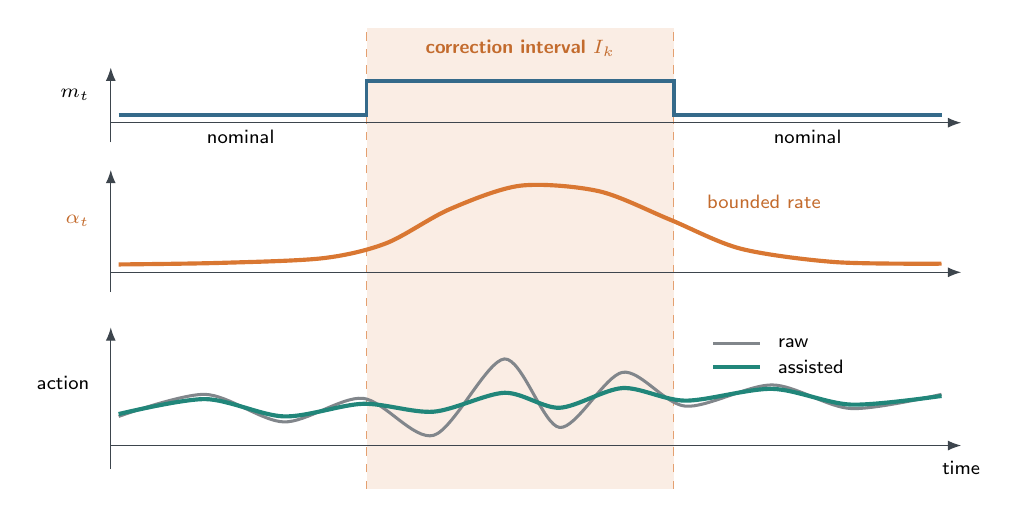
\begin{tikzpicture}[font=\sffamily\scriptsize,>=Latex]
    \def\xmax{10.8}

    % Correction interval background shared by all panels.
    \fill[GainOrange!13] (3.25,-0.3) rectangle (7.15,5.55);
    \draw[GainOrange!70,dashed] (3.25,-0.3) -- (3.25,5.55);
    \draw[GainOrange!70,dashed] (7.15,-0.3) -- (7.15,5.55);
    \node[text=GainOrange!90!black,font=\sffamily\scriptsize\bfseries]
      at (5.2,5.3) {correction interval $I_k$};

    % Interval label.
    \draw[->,draw=DarkGray] (0,4.35) -- (\xmax,4.35);
    \draw[->,draw=DarkGray] (0,4.1) -- (0,5.05);
    \draw[line width=1.3pt,draw=AuditBlue]
      (0.1,4.45) -- (3.25,4.45) -- (3.25,4.88) --
      (7.15,4.88) -- (7.15,4.45) -- (10.55,4.45);
    \node[anchor=east] at (-0.15,4.7) {$m_t$};
    \node[anchor=north] at (1.65,4.38) {nominal};
    \node[anchor=north] at (8.85,4.38) {nominal};

    % Continuous gain.
    \draw[->,draw=DarkGray] (0,2.45) -- (\xmax,2.45);
    \draw[->,draw=DarkGray] (0,2.2) -- (0,3.75);
    \draw[line width=1.5pt,draw=GainOrange]
      plot[smooth] coordinates {(0.1,2.55) (1.4,2.57) (2.7,2.63)
      (3.5,2.82) (4.3,3.25) (5.2,3.55) (6.2,3.48)
      (7.1,3.12) (8.0,2.75) (9.2,2.58) (10.55,2.56)};
    \node[anchor=east,text=GainOrange!90!black] at (-0.15,3.1) {$\alpha_t$};
    \node[anchor=west,text=GainOrange!90!black] at (7.45,3.35)
      {bounded rate};

    % Raw and assisted action schematic.
    \draw[->,draw=DarkGray] (0,0.25) -- (\xmax,0.25);
    \draw[->,draw=DarkGray] (0,-0.05) -- (0,1.75);
    \draw[line width=1.1pt,draw=DarkGray!65]
      plot[smooth] coordinates {(0.1,0.62) (1.2,0.9) (2.2,0.55)
      (3.2,0.85) (4.1,0.38) (5.0,1.35) (5.7,0.48)
      (6.5,1.18) (7.3,0.75) (8.4,1.02) (9.4,0.72) (10.55,0.9)};
    \draw[line width=1.5pt,draw=ActionTeal]
      plot[smooth] coordinates {(0.1,0.65) (1.2,0.84) (2.2,0.62)
      (3.2,0.78) (4.1,0.68) (5.0,0.92) (5.7,0.73)
      (6.5,0.98) (7.3,0.82) (8.4,0.97) (9.4,0.77) (10.55,0.88)};
    \node[anchor=east] at (-0.15,1.05) {action};
    \draw[line width=1.1pt,draw=DarkGray!65] (7.65,1.55) -- (8.25,1.55);
    \node[anchor=west] at (8.35,1.55) {raw};
    \draw[line width=1.5pt,draw=ActionTeal] (7.65,1.25) -- (8.25,1.25);
    \node[anchor=west] at (8.35,1.25) {assisted};

    \node[anchor=north] at (\xmax,0.18) {time};
  \end{tikzpicture}}
  \caption{Schematic relation between interval supervision and continuous
  assistance. Binary interval annotations define an offline training signal;
  the deployed gain remains a bounded, rate-constrained continuous state. The
  action trace is illustrative and does not report experimental data.}
  \label{fig:supervision_gain}
\end{figure}


\subsection{Visual-Conditioned Continuous Action Filter}
At time $t$, the filter uses a causal history of length $L$,
\begin{equation}
  x_t=\{u^{\mathrm{raw}}_{t-L:t-1},q_{t-L:t-1},v_{t-L:t}\},
  \qquad v_t=E_{\mathrm{vis}}(o_t),
  \label{eq:context}
\end{equation}
where the frozen encoder $E_{\mathrm{vis}}$ maps the synchronized camera views
to a continuous representation $v_t$. We use SigLIP2 for this representation.
An offline vision-language auditor processes longer clips and proposes task
phase, progress, stagnation, recovery, and correction events with confidence
scores. Human review converts these proposals into interval labels, terminal
labels, and the admission decision. Online inference uses only the context in
Eq.~\eqref{eq:context}.

Linear projections convert command, state, and visual features into tokens. A
causal Transformer maps their interleaved history to $h_t$ using the attention
mask $M_{ij}=0$ for $j\leq i$ and $-\infty$ otherwise
\citep{vaswaniAttentionAllYou2023}. The action branch models a conditional
expert-action distribution with a conditional variational autoencoder (CVAE)
\citep{kingmaAutoEncodingVariationalBayes2022}:
\begin{align}
  z_t &\sim p_\theta(z_t\mid h_t), \\
  \hat u^{\mathrm{exp}}_t &\sim
  p_\theta(u^{\mathrm{exp}}_t\mid h_t,z_t),
  \label{eq:cvae_action}
\end{align}
with an amortized posterior
$q_\phi(z_t\mid h_t,u^{\mathrm{exp}}_t)$ used during training. The latent
variable represents multiple locally plausible expert actions under similar
visual context.

A separate gain branch maps $h_t$ to a bounded increment and updates a scalar
assistance state,
\begin{align}
  \Delta\alpha_t &= r_\alpha\tanh(g_\theta(h_t)), \\
  \alpha_t &= \operatorname{clip}
  (\alpha_{t-1}+\Delta\alpha_t,0,\alpha_{\max}),
  \label{eq:gain}
\end{align}
where $r_\alpha$ limits the per-step gain change and $\alpha_{\max}$ limits
authority. The candidate expert action defines the local residual and the gain
sets its applied magnitude:
\begin{align}
  \hat\delta_t &= \hat u^{\mathrm{exp}}_t-u^{\mathrm{raw}}_t, \\
  u^{\mathrm{out}}_t &= \Pi_{\mathrm{safe}}\!\left(
  u^{\mathrm{raw}}_t+\alpha_t\hat\delta_t\right).
  \label{eq:composition}
\end{align}
$\Pi_{\mathrm{safe}}$ projects the composed command onto declared joint
position, velocity, and command-rate constraints. The executed action changes
$o_{t+1}$, so Eqs.~\eqref{eq:context}--\eqref{eq:composition} recur on the
resulting visual history.

\subsection{Complementary Supervision}
For synchronized trajectories in $\Aaction$, let
$u^{\mathrm{exp}}_t$ denote the recorded expert command. We optimize
\begin{equation}
  \mathcal{L}=\lambda_a\mathcal{L}_{\mathrm{act}}+
  \lambda_g\mathcal{L}_{\mathrm{gain}}+
  \lambda_n\mathcal{L}_{\mathrm{nom}}+
  \beta\mathcal{L}_{\mathrm{KL}}+
  \lambda_s\mathcal{L}_{\mathrm{smooth}}.
  \label{eq:objective}
\end{equation}
The action term emphasizes expert behavior inside correction intervals,
\begin{align}
  \mathcal{L}_{\mathrm{act}}
  &=\frac{1}{T}\sum_t w_t
  \|\hat u^{\mathrm{exp}}_t-u^{\mathrm{exp}}_t\|_1,\\
  w_t&=1+(w_{\mathrm{corr}}-1)m_t.
  \label{eq:action_loss}
\end{align}
The gain term supplies interval-level trend supervision rather than a target
gain at every frame:
\begin{equation}
\begin{split}
  \mathcal{L}_{\mathrm{gain}}=\frac{1}{T}\sum_t
  \big[&m_t[\alpha_{\min}-\alpha_t]_+\\
       &+(1-m_t)\alpha_t\big],
  \label{eq:gain_loss}
\end{split}
\end{equation}
where $[a]_+=\max(a,0)$ and $\alpha_{\min}$ denotes the minimum useful gain
range selected on validation data. Successful nominal segments further
penalize candidate corrections that would move an already adequate command,
\begin{equation}
  \mathcal{L}_{\mathrm{nom}}=\frac{1}{T}\sum_t(1-m_t)
  \|\hat\delta_t\|_1.
  \label{eq:nominal_loss}
\end{equation}
The CVAE regularizer is
\begin{equation}
  \mathcal{L}_{\mathrm{KL}}=
  D_{\mathrm{KL}}\!\left(q_\phi(z_t\mid h_t,u^{\mathrm{exp}}_t),
  \|,p_\theta(z_t\mid h_t)\right),
\end{equation}
and $\mathcal{L}_{\mathrm{smooth}}$ penalizes adjacent changes in both
$u^{\mathrm{out}}_t$ and $\alpha_t$. This factorization lets the action branch
represent where a plausible local correction leads while the gain branch
controls how much of it enters the command stream.

\subsection{Safe Iterative Data Collection}
Online collection executes the encoder, temporal model, action and gain
branches, and safety projection. Runtime checks cover non-finite outputs,
residual magnitude and rate, joint and velocity limits, model timeout, and
missing visual frames; the operator retains a manual bypass and hardware
emergency stop.

Before round zero, we freeze a reference audit set $H_{\mathrm{ref}}$ and the
admission rule $\Gamma$. At round $r$, dataset $D_r$ trains filter $f_r$, which
collects candidate episodes $D'_r$. A configuration-stratified subset
$H^{(r)}_{\mathrm{audit}}$ is independently re-audited and permanently excluded
from training. The remaining admitted candidates update the next round:
\begin{equation}
\begin{split}
  D_r &\xrightarrow{\mathrm{train}} f_r
  \xrightarrow{\mathrm{collection}} D'_r,\\
  D_{r+1} &=D_r\cup
  \Gamma\!\left(D'_r\setminus H^{(r)}_{\mathrm{audit}}\right).
  \label{eq:flywheel}
\end{split}
\end{equation}
$H_{\mathrm{ref}}$ detects cross-round audit drift, while
$H^{(r)}_{\mathrm{audit}}$ estimates false admission and missed valid episodes
on newly collected data. With $\Gamma$, operator time, reset count, task quotas,
and safety limits fixed, changes in admitted demonstrations per operator minute
measure the practical effect of each update.

\section{Experiments}
\label{sec:experiments}

The evaluation is organized around three questions. \textbf{Q1:} Do correction
intervals and successful nominal segments provide reliable and complementary
supervision? \textbf{Q2:} Does the learned filter preserve adequate human
motion while improving difficult states and unseen configurations?
\textbf{Q3:} Does iterative updating increase valid demonstrations per unit of
operator time, and do those demonstrations improve a downstream policy?
Unless stated otherwise, comparisons use the same robot, control interface,
active operator time, reset count, configuration quota, safety limits, and
episode-level data split.

\subsection{Setup and Evaluation Protocol}
\label{sec:exp_setup}

Each episode contains synchronized RGB observations, raw, filtered, and
executed commands, robot state, audit events, correction intervals, terminal
status, and configuration metadata. Tasks start with a grasped object and a
visually observable target, and include local approach, alignment, correction,
or short-horizon execution. Success tolerances, velocity limits, and safety
termination conditions are fixed before collection. Participants receive the
same familiarization period and use every compared method on matched
configurations in balanced crossover order. The primary collection-efficiency
analysis is paired within novice operators; experienced operators provide a
secondary experience-stratified analysis.

\begin{table}[!t]
  \centering
  \caption{Experimental protocol.}
  \label{tab:protocol}
  \footnotesize
  \setlength{\tabcolsep}{4pt}
  \begin{tabularx}{\columnwidth}{@{}>{\raggedright\arraybackslash}p{0.43\columnwidth}Y@{}}
    \toprule
    Item & Configuration \\
    \midrule
    Robot and end-effector & \\
    Teleoperation interface & \\
    Cameras and placement & \\
    Image resolution / rate & \\
    Control mode / rate & \\
    Synchronization error & \\
    Visual encoder & SigLIP2: \\
    Offline auditor & Qwen-VL: \\
    History $L$; gain limits $\alpha_{\max},r_\alpha$ & \\
    Tasks / configurations & \\
    Episodes per configuration & \\
    Operators (novice / experienced) & \\
    Familiarization / crossover order & \\
    Train / validation / test episodes & \\
    $H_{\mathrm{ref}}$ / round-audit episodes & \\
    Operator-time / reset / safety budgets & \\
    \bottomrule
  \end{tabularx}
\end{table}

All splits are made at the complete-episode level, so adjacent windows from a
single trajectory never cross train, validation, and test sets. The cold-start
round uses manually confirmed action data. Later rounds apply the same
admission rule $\Gamma$ to update $\Aaction$; failed, near-miss, conflicting,
and anomalous episodes remain in $\Aaudit$. Metrics are aggregated within an
episode and then across operators and configurations. We use
\begin{align}
  E_{\mathrm{nom}}&=\frac{1}{|\mathcal{N}|}\sum_{t\in\mathcal{N}}
    \|u^{\mathrm{out}}_t-u^{\mathrm{raw}}_t\|_1,\qquad
  G_{\mathrm{corr}}=\frac{1}{|\mathcal{C}|}\sum_{t\in\mathcal{C}}\alpha_t,\\
  \Delta G&=G_{\mathrm{corr}}-G_{\mathrm{nom}},\qquad
  G_{\mathrm{nom}}=\frac{1}{|\mathcal{N}|}\sum_{t\in\mathcal{N}}\alpha_t,
  \label{eq:exp_metrics}
\end{align}
where $\mathcal{C}=\{t:m_t=1\}$ and $\mathcal{N}=\{t:m_t=0\}$. We also
report action prediction error, gain AUPRC, gain total variation, jerk, latency,
clipping, bypass, and safety events. A threshold $\eta$ is selected on the
validation set and frozen for interval IoU and boundary-delay statistics.

\subsection{Auditable Supervision}
\label{sec:exp_supervision}

Q1 tests both the audit signal and the information supplied by its two episode
parts. A second annotator independently labels correction intervals and
terminal outcomes in the frozen reference set $H_{\mathrm{ref}}$. We report
interval IoU, active-frame F1, boundary error, success/failure agreement,
admission agreement, and review time for manual labels, VLM proposals with
review, and unreviewed proposals. Table~\ref{tab:q1} retains the primary audit
and assistance outcomes; boundary and admission errors are reported alongside
the corresponding intervals in the text. We then train the filter with full,
nominal-only, correction-only, and reviewed-VLM supervision. Action prediction
error and gain AUPRC are secondary diagnostics.

\begin{table}[!t]
  \centering
  \caption{Audit reliability and complementary-supervision ablations.}
  \label{tab:q1}
  \footnotesize
  \setlength{\tabcolsep}{3pt}
  \textbf{(a) Audit reliability and effort}\par\smallskip
  \begin{tabularx}{\columnwidth}{@{}Yccc@{}}
    \toprule
    Audit procedure & IoU $\uparrow$ & F1 $\uparrow$ & Review time $\downarrow$ \\
    \midrule
    Independent manual relabel & & & \\
    VLM proposals + review & & & \\
    VLM proposals & & & \\
    \bottomrule
  \end{tabularx}
  \smallskip
  \textbf{(b) Supervision ablation}\par\smallskip
  \begin{tabularx}{\columnwidth}{@{}Yccc@{}}
    \toprule
    Supervision & $E_{\mathrm{nom}}\downarrow$ & $\Delta G\uparrow$ & $S_{\mathrm{exec}}\uparrow$ \\
    \midrule
    Full complementary supervision & & & \\
    Nominal-only & & & \\
    Correction-only & & & \\
    Reviewed VLM supervision & & & \\
    \bottomrule
  \end{tabularx}
\end{table}

The comparison is intended to show whether nominal successes constrain
unnecessary offsets while correction intervals improve local recovery, rather
than merely increasing the number of training windows.

\subsection{Continuous Assistance and Generalization}
\label{sec:exp_filter}

Q2 compares raw teleoperation, a fixed temporal filter, an action-only
trajectory predictor, and the complete filter. All methods use the same safety
projection and data budget. Results are split between successful nominal
segments and episodes containing correction intervals. We then remove visual
context, merge the action and gain branches, or remove the gain-rate
constraint. The frozen model is then evaluated on unseen object poses and
configurations. Table~\ref{tab:q2} denotes gain total variation by
$V_\alpha$ and execution success by $S_{\mathrm{exec}}$.

\begin{table}[!t]
  \centering
  \caption{Continuous assistance, architecture ablations, and held-out
  generalization.}
  \label{tab:q2}
  \footnotesize
  \setlength{\tabcolsep}{2.5pt}
  \begin{tabularx}{\columnwidth}{@{}Yccccc@{}}
    \toprule
    Method / setting & $E_{\mathrm{nom}}\downarrow$ & $\Delta G\uparrow$ & $V_\alpha\downarrow$ & Jerk $\downarrow$ & $S_{\mathrm{exec}}\uparrow$ \\
    \midrule
    \multicolumn{6}{@{}l}{\itshape Baselines} \\
    Raw teleoperation & & & & & \\
    Fixed temporal filter & & & & & \\
    Action-only trajectory model & & & & & \\
    \method{} (ours) & & & & & \\
    \addlinespace[2pt]
    \multicolumn{6}{@{}l}{\itshape Architecture ablations} \\
    Without visual context & & & & & \\
    Shared action/gain branch & & & & & \\
    Without gain-rate limit & & & & & \\
    \addlinespace[2pt]
    \multicolumn{6}{@{}l}{\itshape Generalization} \\
    In-distribution & & & & & \\
    Unseen configuration & & & & & \\
    \bottomrule
    \end{tabularx}
\end{table}

The primary interpretation is a paired trade-off: $E_{\mathrm{nom}}$ measures
how closely the filter preserves adequate operator input, while $\Delta G$,
$V_\alpha$, jerk, and $S_{\mathrm{exec}}$ characterize assistance around
difficult states. We report means with standard deviations or 95\% confidence
intervals; the final caption specifies the repeated-measures test and unit of
analysis.

\subsection{Fixed-Budget Collection and Downstream Utility}
\label{sec:exp_flywheel}

Q3 compares a static filter, single-round training, and iterative updates under
matched operator active time, reset count, configuration quota, and safety
budget. Every round uses the frozen reference set and admission rule. A
mutually exclusive $H^{(r)}_{\mathrm{audit}}$ is manually reviewed to estimate
admission precision, recall, and conflict rate on newly collected episodes.
The primary quantity is valid-demonstration yield,
\begin{equation}
  \rho_r=\frac{|\Aaction^{(r)}|}
  {\operatorname{operator\ minutes}^{(r)}}.
  \label{eq:yield}
\end{equation}
We train one fixed downstream learner, ACT or Diffusion Policy, with identical hyperparameters on the
admitted data from each round \citep{zhaoLearningFineGrainedBimanual2023,chiDiffusionPolicyVisuomotor2024}.
The downstream split is disjoint from filter training, and downstream results
do not affect data admission.

\begin{table*}[!t]
  \centering
  \caption{Fixed-budget flywheel and downstream utility.}
  \label{tab:q3}
  \footnotesize
  \setlength{\tabcolsep}{3pt}
  \begin{minipage}[t]{0.47\textwidth}
    \centering
    \textbf{(a) Collection yield and audit stability}\par\smallskip
    \begin{tabularx}{\linewidth}{@{}Ycccc@{}}
      \toprule
      Procedure & $\rho_0\uparrow$ & $\rho_1\uparrow$ & $\rho_2\uparrow$ & Audit P/R $\uparrow$ \\
      \midrule
      Static filter & & & & \\
      Single-round training & & & -- & \\
      Iterative flywheel & & & & \\
      \bottomrule
    \end{tabularx}
  \end{minipage}\hfill
  \begin{minipage}[t]{0.47\textwidth}
    \centering
    \textbf{(b) Downstream utility}\par\smallskip
    \begin{tabularx}{\linewidth}{@{}Yccc@{}}
      \toprule
      Data source & Episodes & $S_{\mathrm{test}}\uparrow$ & $N_{\mathrm{target}}\downarrow$ \\
      \midrule
      Raw teleoperation & & & \\
      Static-filter data & & & \\
      Iteration 1 admitted data & & & \\
      Iteration 2 admitted data & & & \\
      \bottomrule
    \end{tabularx}
  \end{minipage}
\end{table*}

Here $S_{\mathrm{test}}$ is held-out policy success and
$N_{\mathrm{target}}$ is the number of admitted episodes needed to reach the
predeclared target performance. Safety events are reported with operator-level
counts and exposure time rather than compressed into the utility table.
Failure, near-miss, recovery, and conflict types are reported separately from
$\Aaudit$ to determine whether iteration changes the composition of rejected
episodes as well as the admitted count. The main claim is supported only when
$\rho_r$ rises without a corresponding drop in audit precision or downstream
utility.

\section{Limitations}
\label{sec:limitations}

The method begins from manually confirmed cold-start data. Correction
boundaries therefore inherit operator reaction delay and annotator judgment.
Independent relabeling, a frozen reference set, and per-round review quantify
this uncertainty but do not remove human audit cost. Offline VLM proposals may
also cease to save review time when task phases are visually ambiguous or the
collection distribution shifts substantially.

Our scope is limited to visually observable, local manipulation after an object
has been grasped. The evaluation does not directly cover grasp acquisition,
long-horizon navigation, persistent occlusion, force-dependent contact without
force sensing, or deformable-object control. Residual bounds, gain-rate limits,
and safety projections remain specific to the robot and task configuration;
consistent action semantics across embodiments remain open.

The participant count, number of tasks, and number of collection rounds bound
the statistical reach of the operator study. ACT and Diffusion Policy measure
utility for the selected downstream learners, but cannot establish equivalent
benefits for every policy architecture or data scale.

\section{Conclusion}
\label{sec:conclusion}

This work studies how audited demonstrations can improve the next round of
real-robot teleoperation data collection. Successful nominal segments constrain
the model to preserve adequate human input, while correction intervals provide
local recovery behavior in difficult states. A visual-conditioned filter then
predicts a candidate expert action and a continuous assistance gain, composing
them through a bounded residual, gain-rate constraint, and safety projection.

The evaluation extends beyond offline action fitting to the collection process
itself. A frozen reference audit set, independent round-wise review, and a fixed
admission rule maintain comparable standards across iterations. Valid
demonstrations per operator minute measure collection efficiency, and downstream
imitation learning measures whether admitted episodes retain training value.
This framework makes the link between auditing, assistance, and recollection
explicit and experimentally testable for visually observable fine manipulation.


\small
\bibliographystyle{IEEEtranMN}
\bibliography{bib_controls,references}
\end{document}
